\chapter{Improvement of Event Selection through IP-based Uncertainty Cuts} % Main chapter title

\label{Chapter4} % For referencing the chapter elsewhere, use \ref{Chapter1} 


The first part of the work presented here is to demonstrate the improvement of event selection by applying cuts based on the uncertainty of the impact parameter (here denoted as IP) -magnitude. Given the lack of precision and well reconstructed events as described in the introduction, it has become crucial to develop filters in order to gain the most information possible from the pions.\\
Mathematically, the problem consists of a 3D vector \textbf{v} (physically the spacial vector of the primary vertex PV), with a given covariance matrix $\boldsymbol{\Sigma}$ encoding the squared uncertainties $\sigma^2_i$ with respect to the PV-vector components and the correlations $\sigma_{ij}$ between them. As for the nature of the processes in the detector, the distribution of these uncertainties can be assumed to be Gaussian, its contour lines describing three-dimensional ellipsoids. This can be easily shown by considering the contour lines of the multivariate normal distribution
\begin{equation}
	G(\boldsymbol{x};\boldsymbol{\Sigma},\boldsymbol{\mu}=\boldsymbol{v}) = \frac{1}{\sqrt{(2\pi)^3\det{\boldsymbol{\Sigma}}}}\exp{\left[-\frac{1}{2}(\boldsymbol{x}-\boldsymbol{v})^T \boldsymbol{\Sigma}^{-1}(\boldsymbol{x}-\boldsymbol{v}) \right]} = C = const.
\end{equation}
and rearranging all the \textbf{x}-independent terms to the right-hand side of the equation yielding
\begin{equation}
	(\boldsymbol{x}-\boldsymbol{v})^T \boldsymbol{\Sigma}^{-1}(\boldsymbol{x}-\boldsymbol{v}) = -2\cdot\ln\left(C\cdot\sqrt{(2\pi)^3\det{\boldsymbol{\Sigma}}}\right)=K>0.
\end{equation}
The inequality holds, since both $\boldsymbol{\Sigma}$ and $\boldsymbol{\Sigma^{-1}}$ are positive definite, defining the ellipsoid, similar to its 2D version shown in Fig. \ref{fig:ellipse}.
\begin{figure}[h]
	\centering
	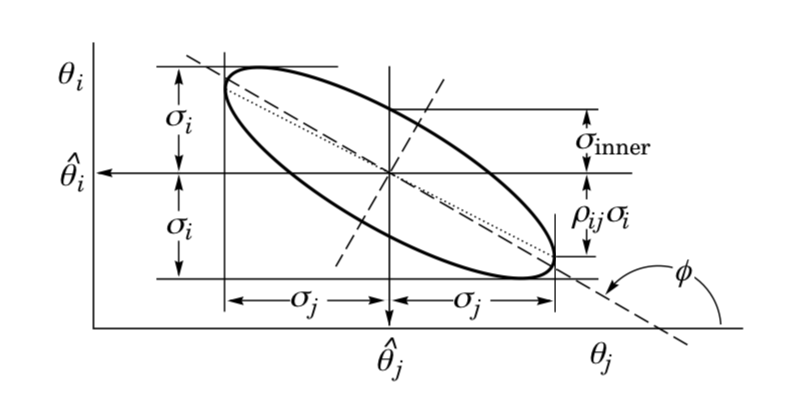
\includegraphics[width=0.7\linewidth]{Figures/ellipsoid}
	\caption{Countour lines of a 2D normal distribution (Source: \parencite{PDG_source})}
	\label{fig:ellipse}
\end{figure}\\
In the following, consider the 3-dimensional impact parameter vector \textbf{d} in the reference frame centred around \textbf{v}. Since the direction of \textbf{d} is the physically important object in the impact parameter method described in section \ref{sec:IP_method}, it is crucial to exclude the cases where the reconstructed IP points to a different direction, giving false results regarding the angle between the $\tau$ decay planes $\varphi^*$. Since these cases are impossible to identify on reconstruction level, one has to apply cuts on the impact parameter based on the uncertainties of \textbf{v}.\\
For this reason, consider the variable $\alpha$, defined as
\begin{equation}
	\alpha = \frac{|\boldsymbol{d}|}{\sigma_{\hat{d}}}.
\end{equation}
This newly defined variable contains information about the magnitude of the IP from the primary vertex expressed in units of the uncertainty $\sigma_{\hat{d}}$. Now one has defined an object, which is suitable for the cuts; it can be assumed that the chance of a more precisely reconstructed impact parameter is higher if it is further away from the uncertainty ellipsoid of the primary vertex.\\
Now it remains to determine $\sigma_{\hat{d}}$. For this, first consider the length of the IP-vector $d$
\begin{equation}
	d = \sqrt{d_x^2+d_y^2+d_z^2}
\end{equation}
with which $\sigma_{\hat{d}}$ can be expressed as through the error propagation formula
\begin{equation}
	\sigma_{\hat{d}} = \mathbf{J}^T \, \boldsymbol{\Sigma} \, \mathbf{J}
\end{equation}
where \textbf{J} denotes the Jacobian defined as
\begin{equation}
	\mathbf{J} = \nabla d
\end{equation}
with the nabla operator acting on the components of \textbf{d}. This yields however
\begin{equation}
	\nabla d = \partial_i \, d \, \boldsymbol{e}_i = \frac{d_i}{d}\boldsymbol{e}_i = \frac{\boldsymbol{d}}{d} = \boldsymbol{\hat{d}},
\end{equation}
meaning the the uncertainty $\sigma_{\hat{d}}$ can be written as
\begin{equation}
	\sigma_{\hat{d}} = \boldsymbol{\hat{d}}^T \, \boldsymbol{\Sigma} \, \boldsymbol{\hat{d}}
\end{equation}
Now it remains to demonstrate the outputs of such a cut which are summarised in Fig. \ref{fig:lambda_dist}-\ref{fig:lambdacuts_CP}. In Fig. \ref{fig:lambda_dist} the distributions of both $d$ and $\sigma_{\hat{d}}$ are portrayed, which then, define the distribution of the cut parameter $\alpha$ shown in Fig. \ref{fig:IP_magOverLambda_dist}. In Fig. \ref{fig:lambdacuts_angles} (for a CP even scenario in the $\mu\rho$ final state), one can immediately observe the filtering of events where the uncertainty is of the same order as the IP itself, leading to smaller differences between the generated and reconstructed data. Similarly promising results can be observed in Fig. \ref{fig:lambdacuts_CP} where one can immediately see the increase in amplitude of the distribution converging to more recognisable $\sin$-like shape.\\
\begin{figure}[h]
	\centering
	\subfigure{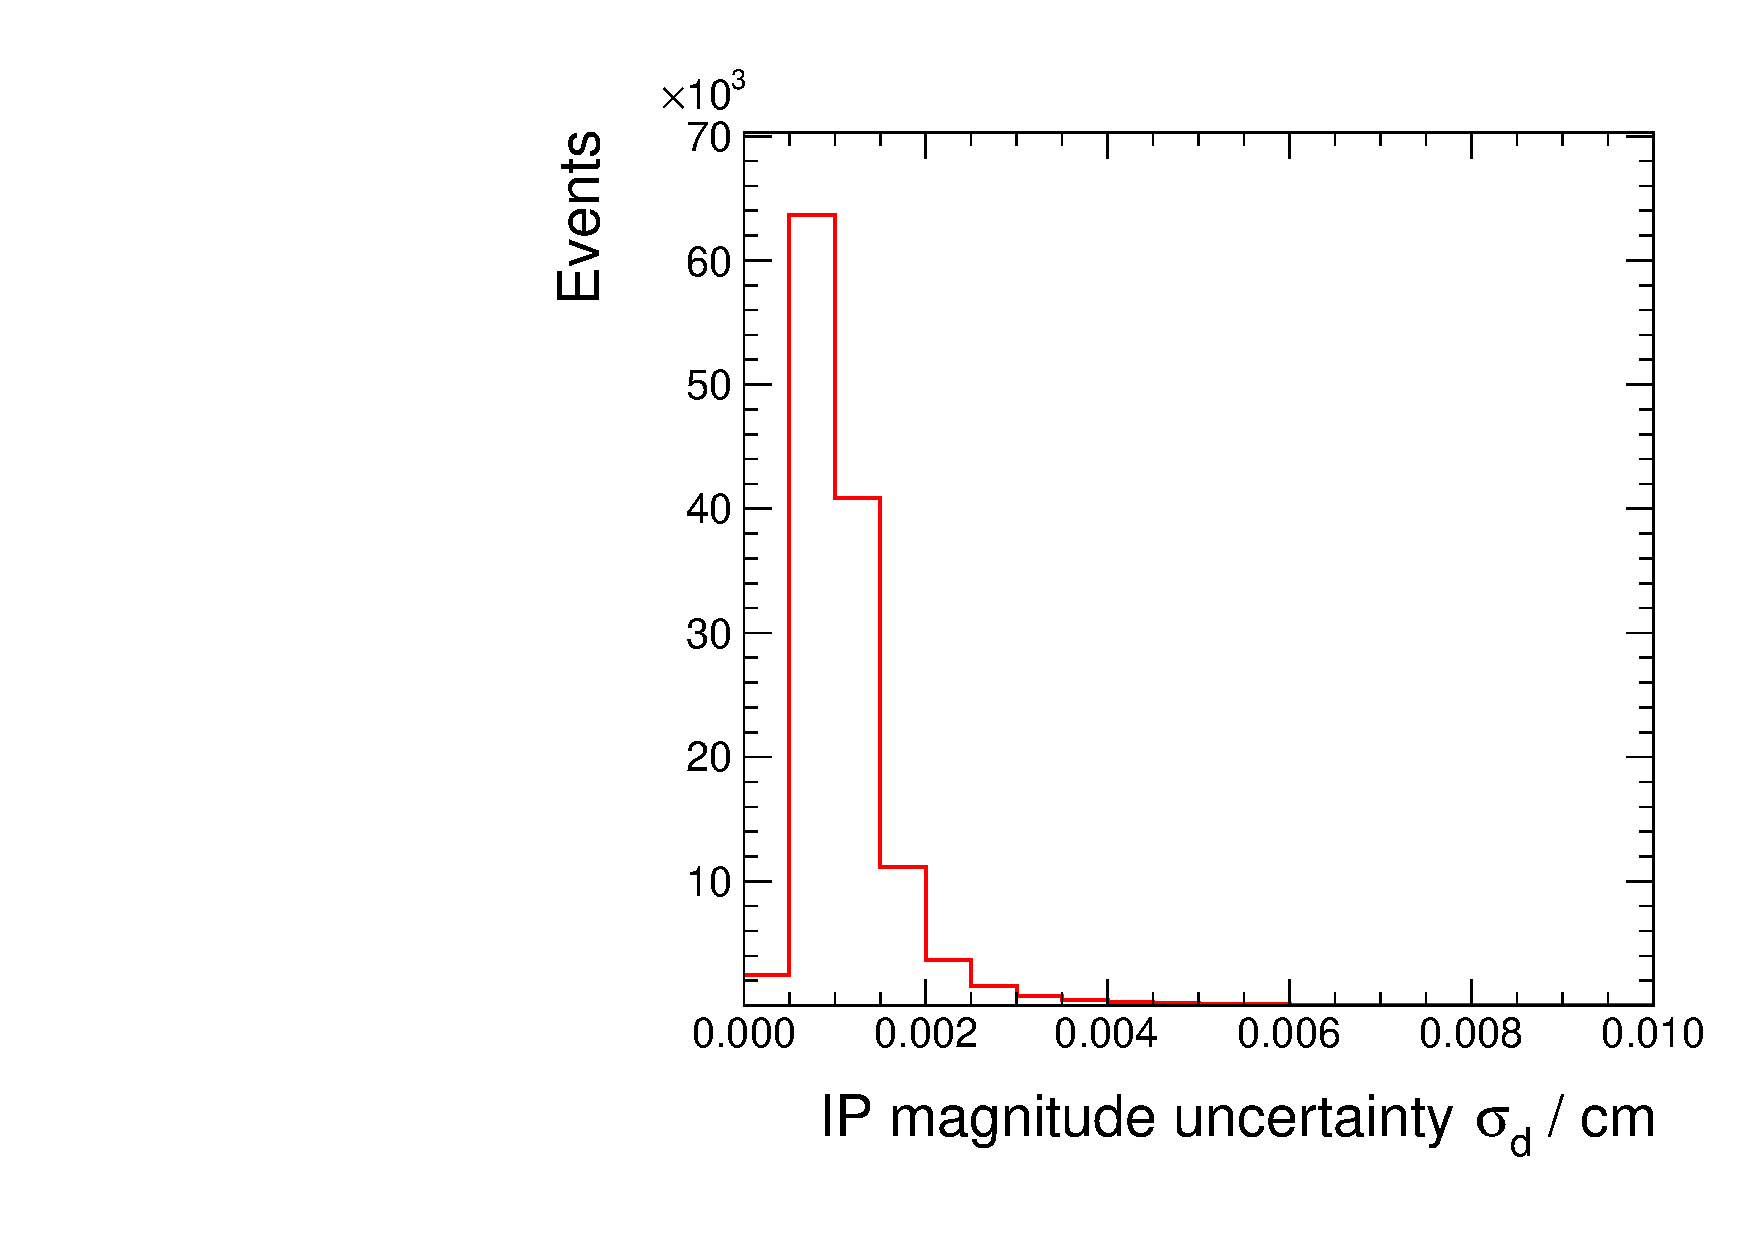
\includegraphics[width=0.4\linewidth]{Figures/IP_mag_err.pdf}}
	\subfigure{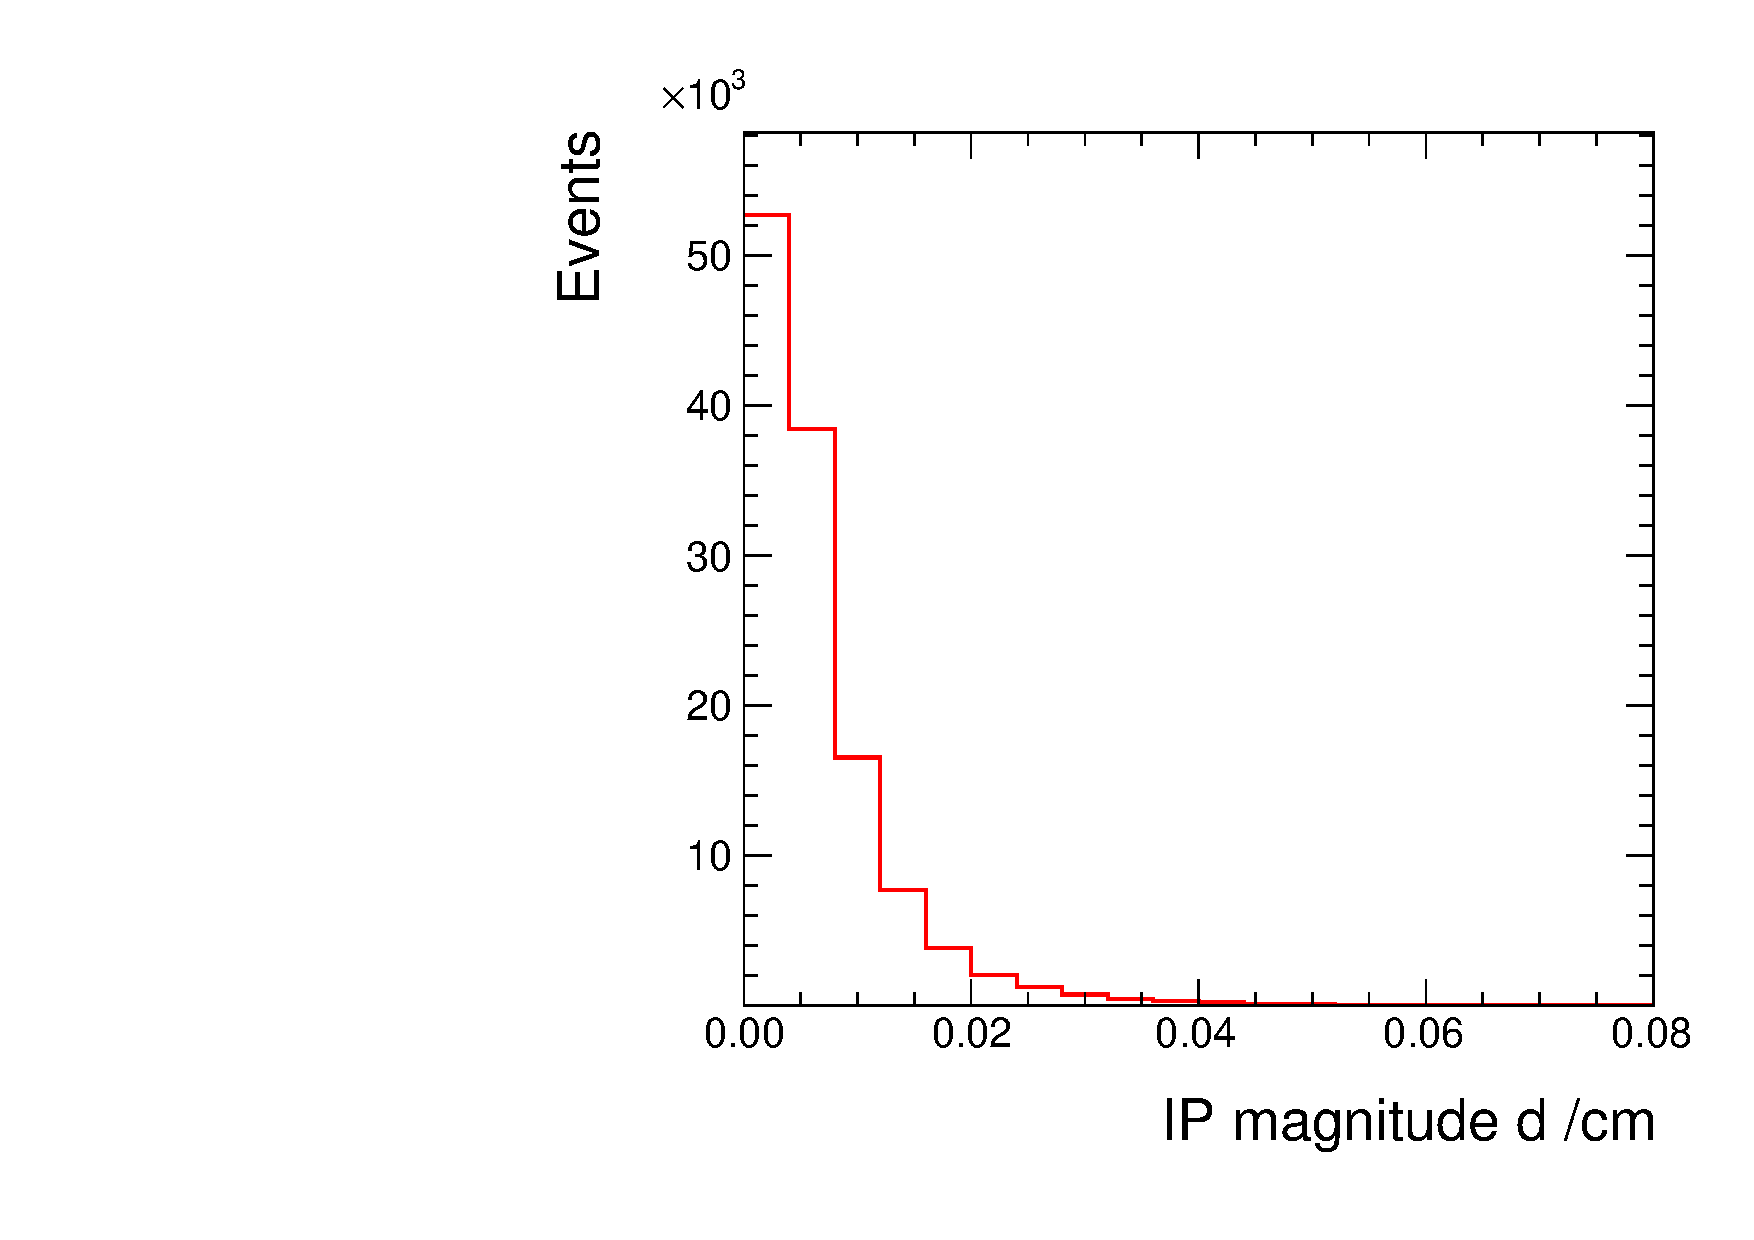
\includegraphics[width=0.4\linewidth]{Figures/IP_mag.pdf}}
	\caption{The Distribution of IP-Vector Magnitudes $d$ and $\sigma_{\hat{d}}$ in the $\mu \, \rho$ decay mode}
	\label{fig:lambda_dist}
\end{figure}
\begin{figure}[h]
	\centering
	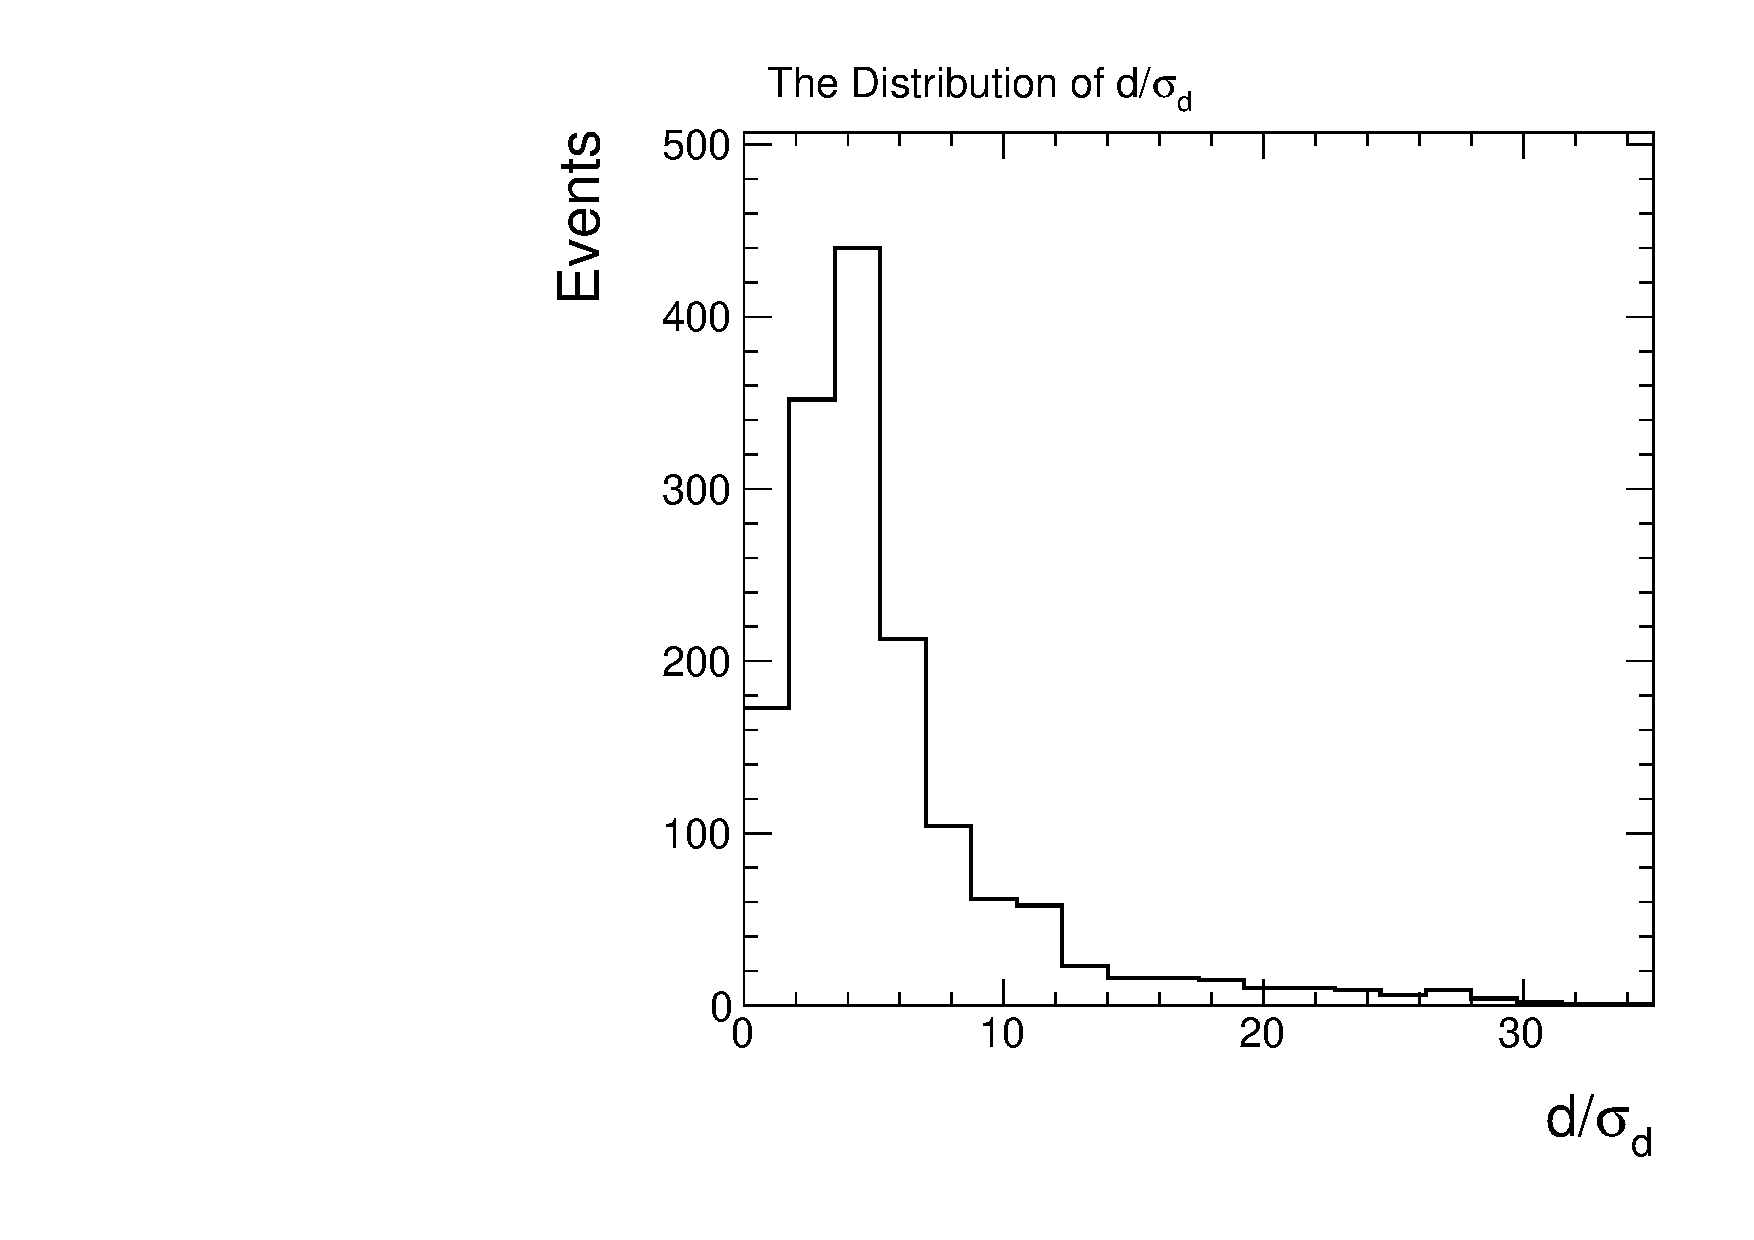
\includegraphics[width=0.7\linewidth]{Figures/IP_mag_IP_Over_err.pdf}
	\caption{The Distribution of IP-vector Magnitudes $d$ in the $\mu \, \rho$ decay mode}
	\label{fig:IP_magOverLambda_dist}
\end{figure}
\begin{figure}[h]
	\centering
	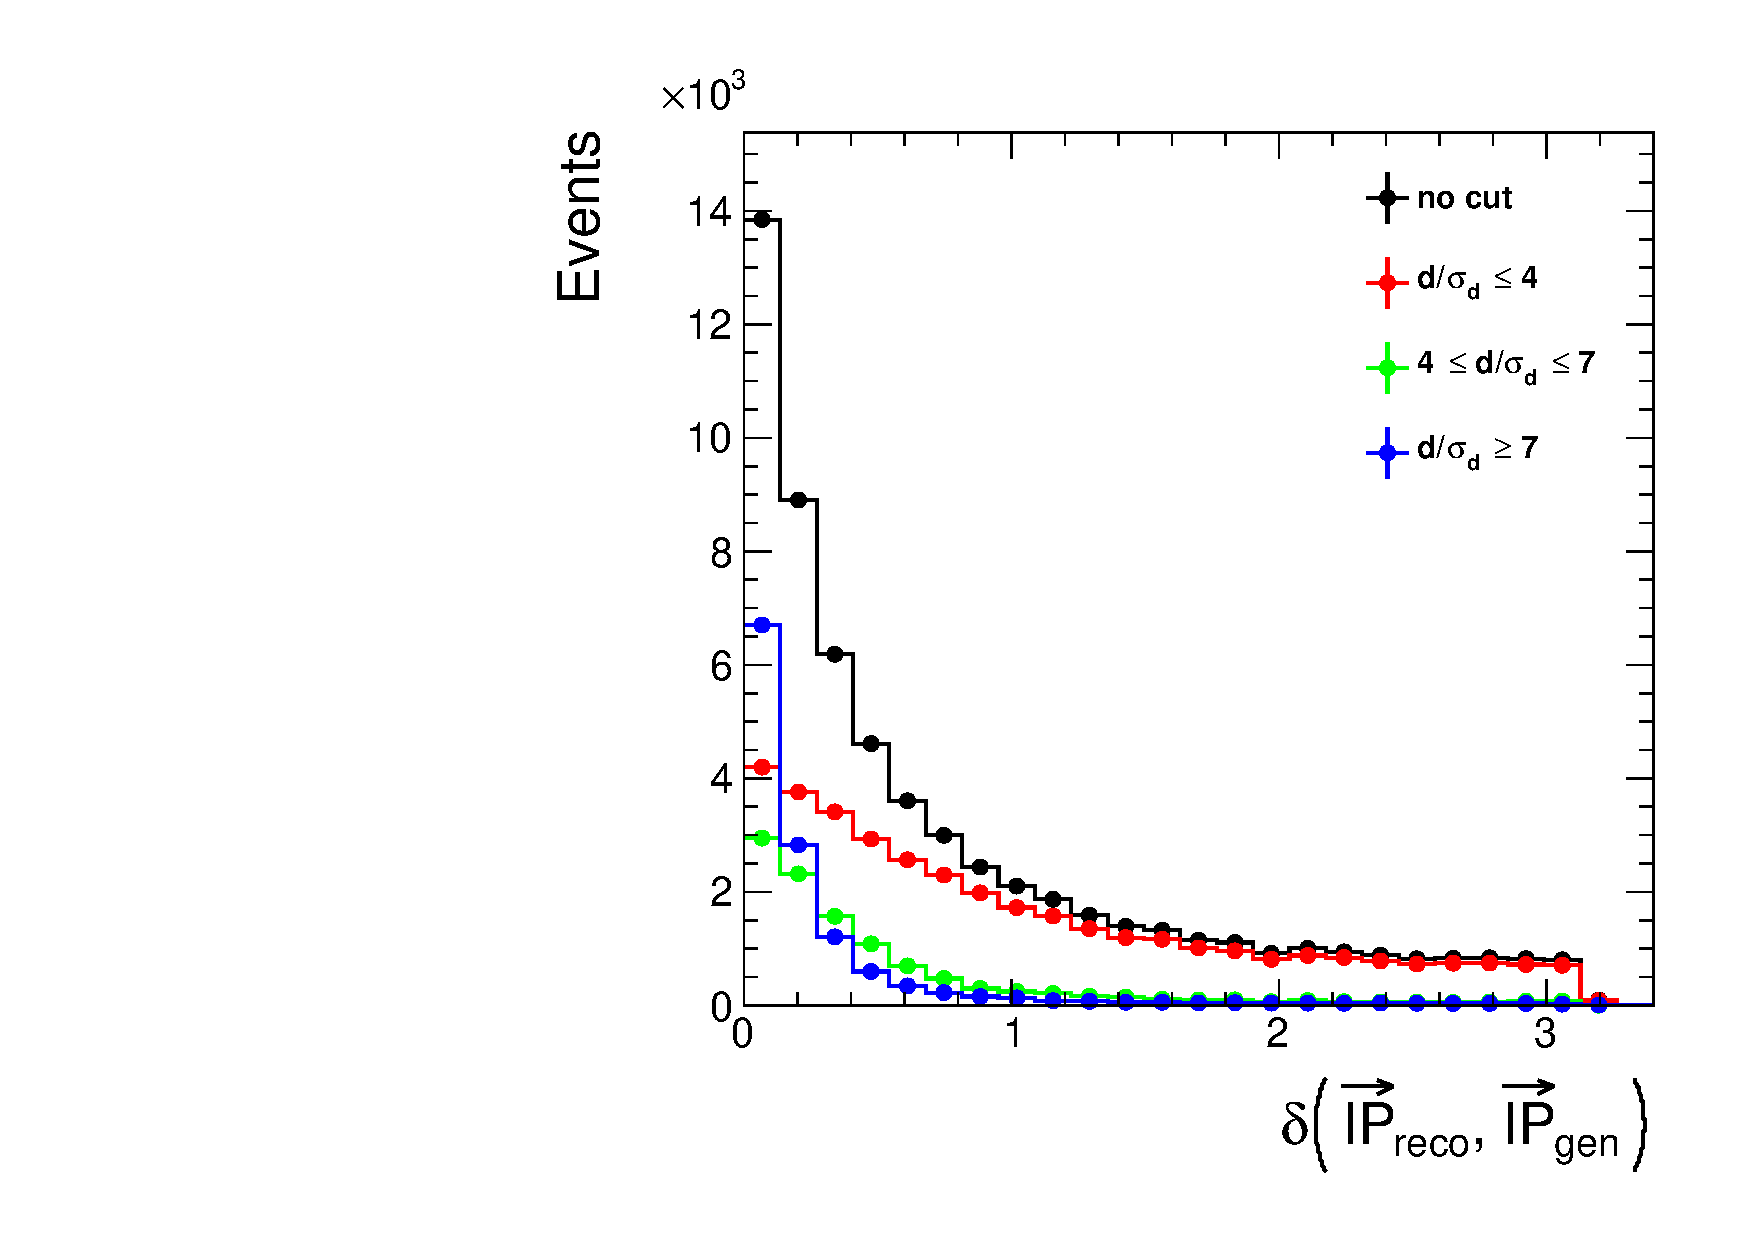
\includegraphics[width=0.7\linewidth]{Figures/deltaGenRecoIP1.pdf}
	\caption{The study of the 3D angle between the generated and reconstructed IP vectors in the $\mu \, \rho$ decay mode}
	\label{fig:lambdacuts_angles}
\end{figure}
\begin{figure}[h]
	\centering
	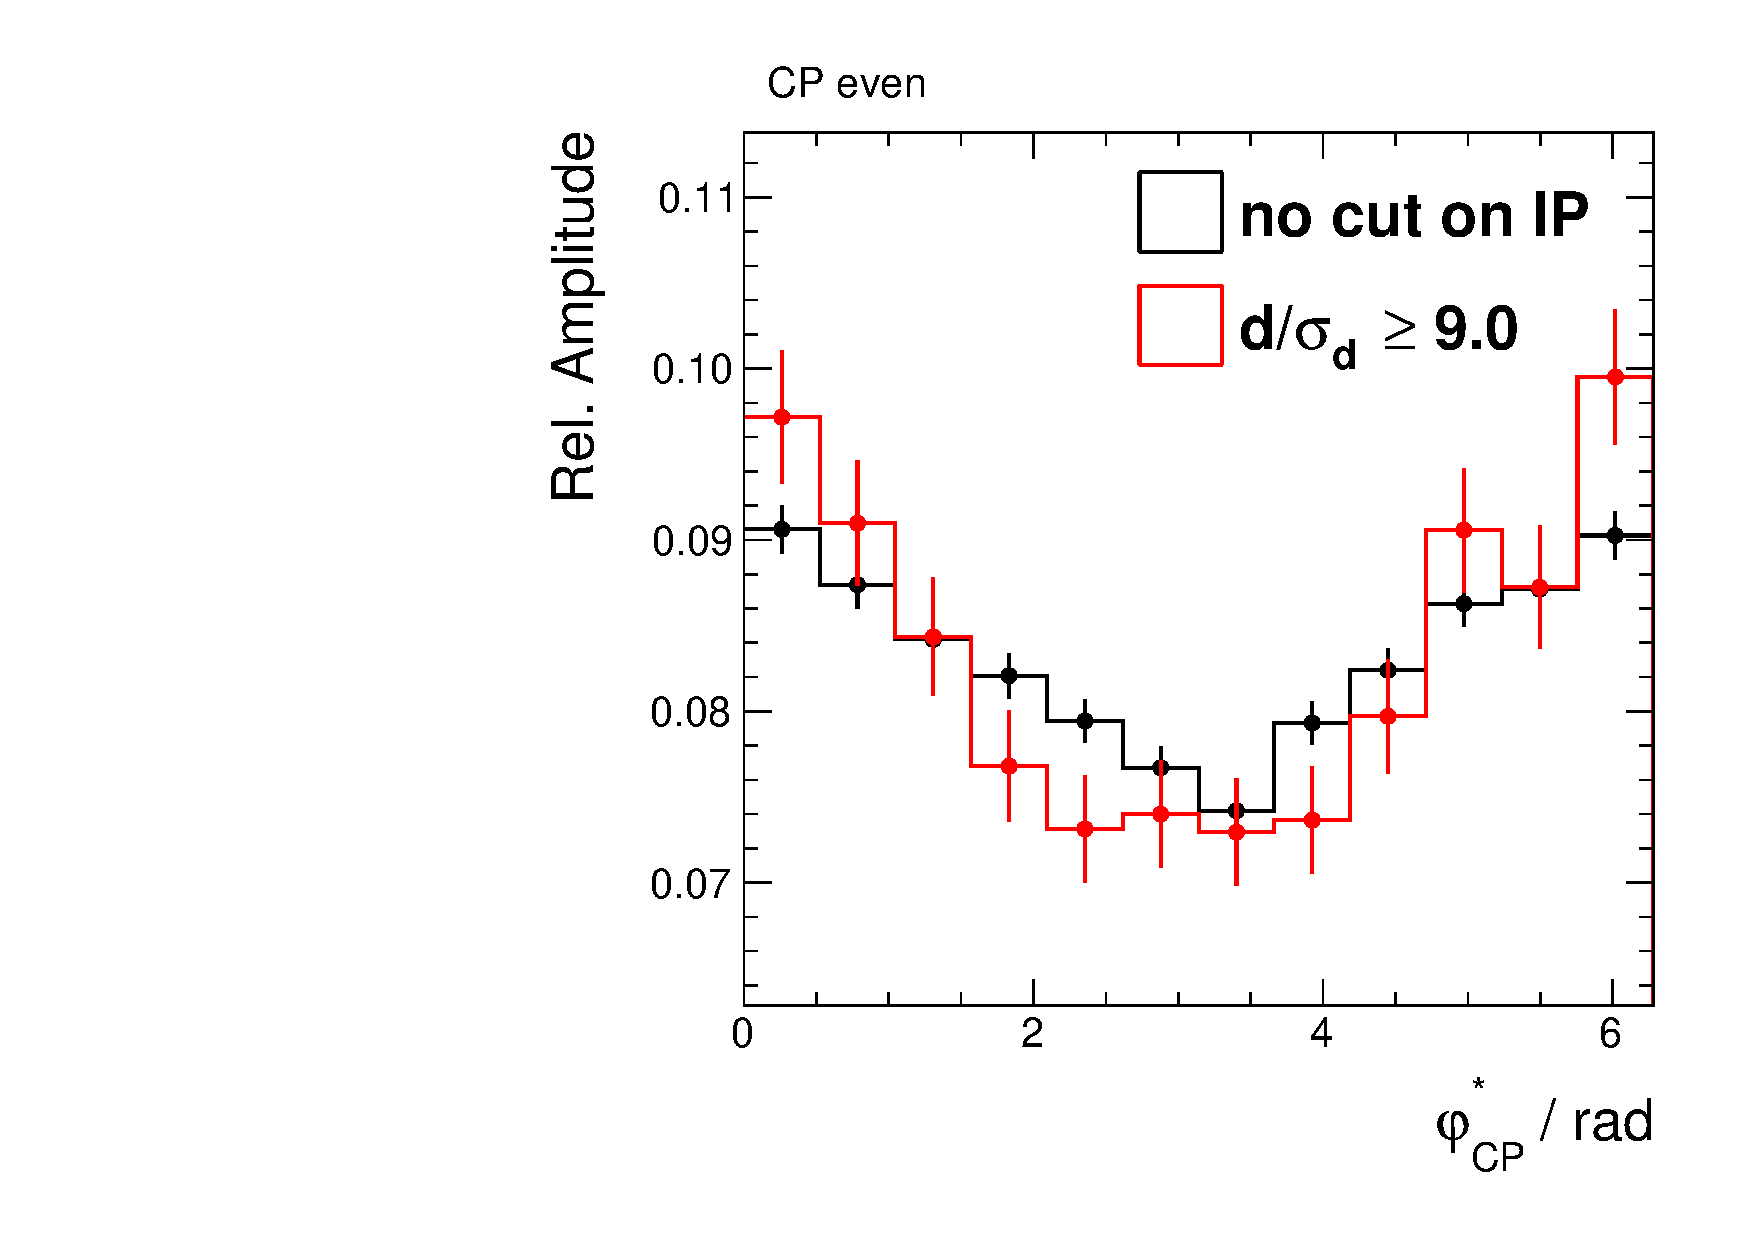
\includegraphics[width=0.7\linewidth]{Figures/recoPhiStarCPCombMerged_norefit_CPeven.pdf}
	\caption{The improvement of data through different cuts for the CP-even scenario in the $\mu \, \rho$ decay mode}
	\label{fig:lambdacuts_CP}
\end{figure}\\
To summarise, an efficient way of event selection has been found, which helps to reduce the influence of the primary vertex uncertainty ellipsoid concerning the direction of the IP vector. In order to complete the analysis, one should not neglect the uncertainty ellipsoid around the "other end" of the PV vector, which corresponds to a point on the track of the particle. Such an additional term however would only increase the total uncertainty with respect to $\sigma_{\hat{d}}$ and therefore its influence.